\chapter{Seitenkanalangriffe}
\label{sec:seitenkanalangriffe}
Lange wurden in der Kryptographie die einzelnen Komponenten als Black
Box betrachtet. Man ist davon ausgegangen, dass eine solche Komponente
lediglich definierte Eingaben, wie z.B. Klartext und Schlüssel, bekommt,
um daraus eine definierte Ausgabe zu berechnen. Praktisch kommen jedoch
weitere Eingaben (Strom), weitere Ausgaben (elektromagnetische
Abstrahlung) sowie interne Zustände (und dadurch andere Laufzeiten)
hinzu, die einem Angreifer Informationen über das Geheimnis der
Komponente liefern können. Es gibt eine ganze Reihe solcher
\emph{Seitenkanäle}, die Informationen nach außen tragen
können. Beispiele hierfür sind:
\begin{itemize}
\item Stromverbrauch
\item Laufzeiten
\item Elektromagnetische Abstrahlung
\item Akkustische Abstrahlung
\end{itemize}

Die Erkenntnis, dass solche Phänomene geeignet sind, Geheimnsse einer
Implementierung von kryptographischen Verfahren preis zu geben, ohne
dass das Verfahren an sich unsicher ist, hat seit der Mitte der 1990er
Jahren zu einer intensiven Beschäftigung mit diesem Problem geführt. 

In diesem Kapitel werden einige grundlegende Angriffe und Gegenmaßnahmen
für Seitenkanalangriffe dargestellt. Die Erklärungen sind dabei nur als
vereinfachte Veranschaulichungen zu sehen und sollen keine umfassende
Beschreibung darstellen.

Man unterscheidet grob zwischen passiven und aktiven
Seitenkanalangriffen. Bei passiven Angriffen misst man Eigenschaften des
normal laufenden Systems, um Rückschlüsse über das Geheimnis ziehen zu
können. Als Beispiel für passive Angriffe werden im folgenden die Simple
und Differential Power Analysis etwas detaillierter erklärt. Bei aktiven
Angriffen nimmt der Angreifer zusätzlich Einfluss auf das System. Dabei
ist von Überhitzen, Übertakten, Einfrieren bis hin zum gezielten
Zerstören von Teilen des Systems alles denkbar. Als Beispiel hierfür
werden Cold Boot Attacks vorgestellt. 

\section{Simple Power Analysis}
\label{sec:simple-power-analys}
Ein einfacher Seitenkanalangriff ist die \emph{Simple Power
  Analysis(SPA)}. Dabei wird der Stromverbrauch einer CPU gemessen,
während diese einen Algorithmus ausführt. Als Beispiel wird im folgenden
untersucht, wie mittels einer SPA der geheime Schlüssel bei einer naiven
RSA-Implementierung gefunden werden kann. Natürlich funktionieren SPAs
aber auch bei vielen anderen Algorithmen.
\subsection{SPA der RSA-Entschlüsselung}
Wird ein RSA-Chiffrat entschlüsselt, so wird \[\plaint
  =\ciphert^d \mod N\] berechnet. Eine gängige Implementierung ist das
Square-and-Multiply-Verfahren in Algorithmus \ref{alg:Square-and-Multiply}. 
\begin{algorithm}[!h]
\caption{Square-and-Multiply-Verfahren}
\label{alg:Square-and-Multiply}
\begin{algorithmic}
\Procedure{SaM}{$x, b$}\Comment{Berechnet $x^k \mod N$, wobei $b$ die
  Binärdarstellung von $k$ ist}

  \State $x \gets C$
  \State $z \gets 1$
  \For{$i\text{ in }\{0, \dots, n-1\}$}
    \If{$b[i]==1$}
      \State $z \gets z \cdot x \mod N$
    \EndIf
    \State $x \gets x^2 \mod N$
  \EndFor
  \State \textbf{return} $z$
\EndProcedure
\end{algorithmic}
\end{algorithm}

Hierbei wird $d$ bitweise abgearbeitet. Je nach dem, ob das $i$-te Bit
von $d$ gleich $1$ oder $0$ ist, werden eine oder zwei Multiplikationen
durchgeführt. Ergibt eine Messung des Stromverbrauchs also einen Verlauf
wie in Abb. \ref{abb:power-attack}, so könnte man daraus schließen,
dass zuerst eine $0$ und dann eine $1$ im Schlüssel verarbeitet wurde,
da zwei Multiplikationen zu einem höheren Stromverbrauch führen, als nur
eine Multiplikation.

\begin{figure}[h]
  \centering
  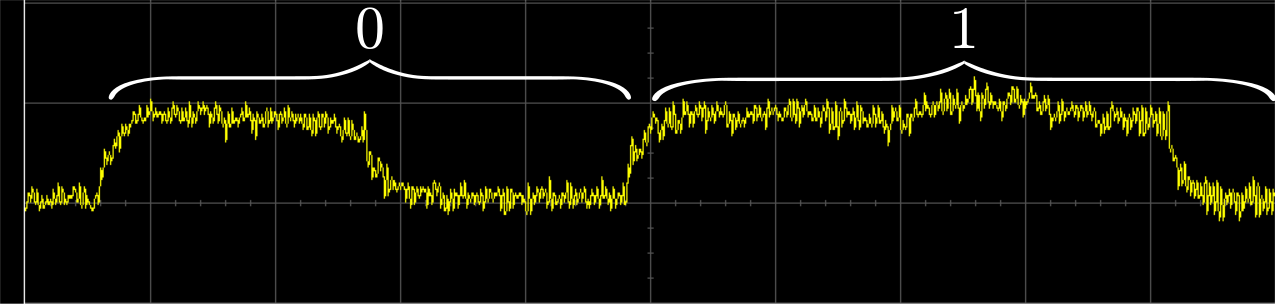
\includegraphics[width=\textwidth]{images/Power_attack}
  \caption{Messung des Stromverbrauchs für SPAs. Quelle: \url{https://commons.wikimedia.org/wiki/File:Power_attack.png}}
  \label{abb:power-attack}
\end{figure}

\subsection{Gegenmaßnahmen}
Um SPAs zu vermeiden, bieten sich Gegenmaßnahmen auf Hardware- und
Algorithmusseite an. Hardwareseitig kann man den Stromverbrauch
unabhängig von den ausgeführten Opereationen konstant halten. Zudem kann
man die Algorithmen so implementieren, dass keine bedingten Sprünge
in Abhängigkeit vom Geheimnis gibt. Außerdem können Dummy-Berechnungen
genutzt werden, um den Stromverbrauch und die Laufzeit  zu verrauschen.

\section{Differential Power Analysis (DPA)}
Eine aufwändigere, aber mächtigere Technik, um aus Power-Traces
Informationen über einen geheimen Schlüssel zu gewinnen, ist die
\emph{Differential Power Analysis (DPA)}. DPA ist auf viele Arten von
Verfahren anwendbar, im Folgenden werden wir beispielhaft das grobe
Vorgehen anhand von Verschlüsselungsverfahren erklären. Um eine DPA
durchführen zu können, muss der Angreifer die Implementierung des
Algorithmus kennen, der auf dem Prozessor läuft. Auserdem braucht er
eine möglichst große Menge an Trace-Message-Paaren $(T_X, X)$, also
jeweils den Stromverbrauch bei der Entschlüsselung einer gegebenen
Nachricht $X$ (oder eines gegebenen Chiffrats).
Ein Angreifer rät nun einen Teil $s$ des Geheimnis $S$, im
Verschlüsselungsbeispiel ist $s$ ein Teil des Secret Keys. Dann
simuliert er den Algorithmus für alle $X$ aus seinen
Trace-Message-Paaren und sortiert die Eingaben in zwei Gruppen \calL,
\calH, wobei
\begin{eqnarray*}
\calL & := &\{X| \texttt{Simulation mit $X$ hat einen niedrigen
  Stromverbrauch}\},\\
\calH & := &\{X| \texttt{Simulation mit $X$ hat einen hohen
  Stromverbrauch}\}.
\end{eqnarray*}
Anschließend betrachtet der Angreifer den durchschnittlichen
\textit{realen} Stromverbrauch beider Gruppen. War $s$ richtig geraten,
so sollte sich der reale Durschnittsverbrauch beider Gruppen stark
unterscheiden. Tut er dies nicht, so war $s$ wohl falsch
geraten. Mithilfe von statistischen Methoden kann ein Angreifer bei
mehrfahre Ausführung von DPAs effizient Informationen über das Geheimnis
errechnen. 

\subsection{Gegenmaßnahmen}
Um sich von DPAs zu schützen, kann man versuchen, den Stromverbrauch
durch zusätzliche Berechnungen zu verrauschen. Beispielsweise kann eine
RSA-Entschlüsselung vorgenommen werden, indem man statt $M = C^D \mod N$
ein zufälliges $R$ wählt und $\frac{(R*C)^D}{R^D} = M \mod N$ berechnet. Durch das
jeweils zufällig gewählte R wird die Entschlüsselung verrauscht, sodass
der Stromverbrauch nicht nur noch abhängig von M ist. Somit kann ein und
das selbe Chiffrat bei mehrfacher Entschlüsslung zu stark verschiedenen
Stromverbräuchen führen. 

\section{Cold Boot Attacks}
\emph{Cold Boot Attacks} machen es sich zunutze, dass der Hauptspeicher
Informationen erst langsam verliert, wenn die Stromversorgung
unterbrochen wird. Die Zeit, die es braucht, bis die Daten verloren
sind, lässt sich beträchtlich hinauszögern, wenn der Speicher (z.B. mit
flüssigem Stickstoff) heruntergekühlt wird. Damit kann der Zeitraum für
einen Angriff von einigen Sekunden auf mehrere Stunden gestreckt werden
\cite{Halderman08}.

\begin{figure}[h]
  \centering
  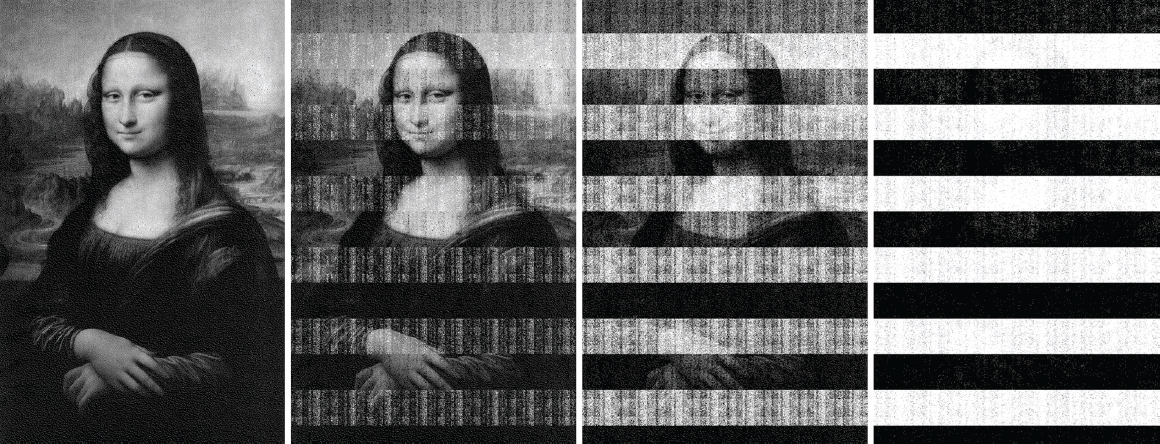
\includegraphics[width=\textwidth]{images/mona-lisa.jpg}
  \caption{Informationsverlust im Hauptspeicher nach 5, 30 und 60 Sekunden sowie nach 5
    Minuten ohne Stromzufuhr. Quelle: \cite{Halderman08}.}
  \label{fig:mona-lisa}
\end{figure}

Setzt ein System eine Festplattenverschlüsselung ein, so muss der
Schlüssel im Speicher gehalten werden, da der Benutzer nicht bei jedem
Fesplattenzugriff nach dem Schlüssel gefragt werden kann. Wenn ein
Angreifer jetzt das System im laufenden Betrieb in seinen Besitz bringt,
kann er den Hauptspeicher herunterkühlen und den Strom abstellen, ohne
das System herunterzufahren. So hat das Betriebssystem nicht die
Möglichkeit, die entsprechenden Speicherbereiche zu überschreiben. Jetzt
kann der Angreifer auf dem Hauptspeicher ein minimales System starten,
dass möglichst wenig Speicher braucht. Dieses minimale System hat die
Möglichkeit, die Speicherbereiche auszulesen, in denen der Schlüssel
gespeichert war. Damit kann der Angreifer dann die Festplatte
entschlüsseln.

\subsection{Gegenmaßnahmen}
Gegen Cold Boot Attacks gibt es Ansätze auf verschiedenen Ebenen. Auf
Ebene des BIOS gibt es die Möglichkeit, dass das BIOS bei jedem Start
den Hauptspeicher neu initialisiert und dabei bestehende Daten
löscht. Damit ist sichergestellt, dass eine Cold Boot Attack nicht vom
eigenen Rechner stattfindet.

Eine weitere Möglichkeit besteht darin, den Schlüssel nicht im
Hauptspeicher, sondern im Prozessor-Cache zu speichern. Der Cache ist,
im Gegensatz zum Hauptspeicher, nicht einzeln entnehmbar und durchläuft
beim Start des Prozessors eine Initialisierung, die die Inhalte des
Caches überschreibt. Dieser Ansatz führt jedoch zu massiven
Leistungseinbußen, da große Teile des Caches für andere Informationen
nicht mehr zur Verfügung stehen.
\section{Theoretische Modelle}
Viele Gegenmaßnahmen gegen Seitenkanalangriffe sind \glqq
Ad-hoc\grqq-Ansätze, die nicht auf formalen Methoden
basierenund meist nicht gut untersucht sind. Wünschenswert sind aber Systeme, deren Sicherheit beweisbar
ist. Dafür möchte man die Eigenschaft eines Systems, sicher gegenüber
Seitenkanalangriffen zu sein, in einem formalen Modell darstellen
können. Solche Modelle sind Gegenstand aktueller Forschung. Theoretische
Modelle gegen solche Seitenkanalangriffe werden hier nur oberflächlich
behandelt. Als Einstieg für eine tiefere Beschäftigung mit dem Thema
bietet sich \cite{mol2010} an.

Um Seitenkanäle zu beschreiben, verwendet man beispielsweise eine
\emph{Leakage}-Funktion. Eine solche Funktion beschreibt, welche
Informationen eine Implementierung nach außen gibt. Die Ausgabe hängt ab
vom internen Zustand $S$, einer Eingabe $Y$ sowie einem zufälligen
Rauschen $R$. Darauf aufbauend werden dann verschiedene Arten von
Angriffen unterschieden. 

Die Modelle sind dabei ähnlich zu den uns schon bekannten
Sicherheitsbegriffen wie IND-CPA oder EUF-CMA. Zusätzlich erhält der
Angreifer aber Zugriff auf ein Leakage-Orakle, an das er
Leakage-Funktionen senden kann. 
\subsection{Unbounded (continuous) computational-leakage}
Hierbei werden Informationen durch Prozessoroperationen nach Außen
getragen. Dabei geht man davon aus, dass nur Informationen, die im
Prozessor verarbeitet werden, von außen gelesen werden können. Solche
Angriffe sind die oben beschriebenen Techniken SPA und DPA.

Es wird davon ausgegangen, dass der Algorithmus, der auf der Hardware
läuft, rundenbasiert berechnet wird. Modelliert wird ein Angriff
dadurch, dass sich der Angreifer vor der $i$-ten Runde eine
Leakage-Funktion $f_i$ wählt und nach der $i$-ten Runde $f_i(S_{i-1})$
erhält, wobei $S_{i-1}$ der interne Zustand der Komponente zum
Zeitpunkt $i-1$ ist. Diesen Satz umschreiben: Dabei muss man bei den
Modellen sicherstellen, dass der Angreifer genug Informationen durch
Leakage-Funktionen erhalten kann, um realisischte Angriffe modellieren
zu können, ohne dass der Angreifer trivial das komplette Geheimnis durch
die Leakage-Anfragen erfragen kann. 

Ein Verfahren ist hier sicher, wenn die gewünschte
Sicherheitseigenschaft, die beispielsweise ein modifizerter
IND-CPA-Begriff, auch bei Zugriff auf solche Informationen durch
Leakage-Funktionen über das Geheimnis nicht effizient brechen können. 
\subsection{Memory-Leakage Attacks}
Mit dem oben beschriebenen Modell wird eine wichtige Klasse von
Seitenkanalangriffen nicht modelliert. Cold Boot Attacks können
beispielsweise Informationen leaken, die nicht im Prozessor verarbeitet
wurden. Sicherheit gegen solche und ähnliche Angriffe kann im
sog. \emph{l-(N)AMA-CPA}-Modell beschrieben werden. Dies steht für
\emph{l-boundet (Non-)Adaptive-Memory-Attack-CPA} und erweitert das
IND-CPA-Modell. Der Angreifer bekommt hierbei zugriff auf ein
\emph{Leakage-Orakel} $\mathcal{O}_{sk}$. An dieses darf er $Q$ viele
Funktionen $f_1, \dots, f_q$ schicken und bekommt jeweils $f_i(sk)$
zurück. Dabei gibt es eine Schranke $l$, sodass gilt:
\[
|\sum_{i=1}^Q f_i(sk)|\leq l
\]
Nun gibt es zwei Sicherheitsspiele. Für $l$-NAMA-CPA wird ein
Schlüsselpaar generiert. Dann wählt sich der Angreifer seine Funktionen
$f_i$ und gibt diese an das Orakel. Er bekommt die $f_i(\skey)$ und den
öffentlichen Schlüssel. Ein Verfahren ist $l$-NAMA-CPA-sicher, wenn der
Angreifer mit diesem Wissen nur vernachlässigbar besser durch bloßes
Raten sagen kann, ob in einem Chiffrat, dass mit dem Schlüsselpaar
verschlüsselt wurde, eine 1 oder eine 0 verschlüsselt wurde.

Das Sicherheitsspiel für $l$-AMA-CPA-Sicherheit läuft sehr ähnlich ab,
jedoch bekommt der Angreifer den öffentlichen Schlüssel bevor er das
Orakel anfragt. Außerdem darf er seine Funktionen in Abhängigkeit der
bisher erhaltenen Antworten des Orakels wählen.


\section{Weitere Angriffsmöglichkeiten}
Es gibt noch eine Vielzahl weiterer Seitenkanäle, über die Angriffe
möglich sind. So kann ein Angreifer durch manipulative Telefonanrufe, in
denen er sich als Mitarbeiter ausgibt, Passwörter erlangen. Hierdurch
werden technische Sicherheitsmaßnahmen umgangen. Solche Angriffe, die
sozialer Interaktion beruhen, werden als \emph{social engineering}
bezeichnet.

Ein weiterer verbreiteter Angriffstyp sind \emph{timing attacks}. Hier
nutzt der Angreifer aus, dass ein System je nach Eingabe verschiedene
Laufzeiten hat. Daraus kann ein Angreifer über statistische Methoden
Informationen über den internen Zustand des Systems gewinnen.

Viele technische Geräte sind nicht gegen elektromagneische Abstrahlung
abgeschirmt. Insbesondere Röhrenbildschirme strahlen in Abhängigkeit vom
dargestellten Bild spezifische Strahlung (oft als
\emph{TEMPEST}-Strahlung bezeichnet) ab. Diese kann dazu genutzt werden,
den Bildschirminhalt zu berechnen und damit Inhalte abzugreifen, bevor
sie verschlüsselt werden.

Denkbar sind auch noch viele weitere Angriffsvektorn, wie
z.B. Temperatur, Geräusche, Spiegelungen, Schwingung durch Tastaturanschläge usw.,
auf die hier nicht näher eingegangen werden kann. 


\section{Fazit}
Seitenkanalangriffe sind eine wichtige Klasse von Angriffen gegen
Implementierung von kryptographischen Komponenten. Sie sind aber nur
schwer mit formalen Methoden in den Griff zu bekommen. Insbesondere
erforden sie neben Kenntnissen aus der formalen Kryptographie auch ein
gutes Verständnis der physikalischen Systeme, der Elektrotechnik etc.
Sie zu analysieren erfordert Kenntnisse in den theoretischen Aspekten
von Kryptographie, in der Implementierung von kryptographischen
Komponenten sowie in den Eigenschaften der Hardware, auf denen die
Komponenten eingesetzt werden.